
\begin{frame}{Diffuse và Denoise thông thường}
    %\begin{columns}
    %	\begin{column}[T]{0.5\textwidth}
    %	
    %	\end{column}
    %	
    %	\hspace*{-1em}
    %	
    %	\begin{column}[T]{0.5\textwidth}
    %		
    %	\end{column}
    %\end{columns}
    
    \textbf{Diffuse}: Cho $\{\alpha_t \in (0, 1)\}_{t=1}^T$ và $\alpha_1 > \alpha_2 > \dots > \alpha_T$.
    
    Với nhiễu:  $\boldsymbol{\epsilon}_{0}, \boldsymbol{\epsilon}_{1}, \dots \boldsymbol{\epsilon}_{T} \sim \mathcal{N}(\mathbf{0}, \mathbf{I});$
    $\boldsymbol{\epsilon}_i \neq \boldsymbol{\epsilon}_j \ (\forall i, j \in T) $, nhiễu $\epsilon_t$ cố định.
    \vspace{-25pt}
    
    \begin{equation}
        \mathbf{x}_t=\sqrt{\alpha_t} \cdot \mathbf{x}_{t-1}+\sqrt{1 - \alpha_t} \cdot \epsilon
    \end{equation}
    \vspace{-15pt}
    
    %	\[
    %	q(x_t | x_{t-1}) = \mathcal{N}(x_t; \sqrt{1 - \beta_t} \, x_{t-1}, \beta_t \, I)
    %	\]
    \begin{figure}
        \centering
        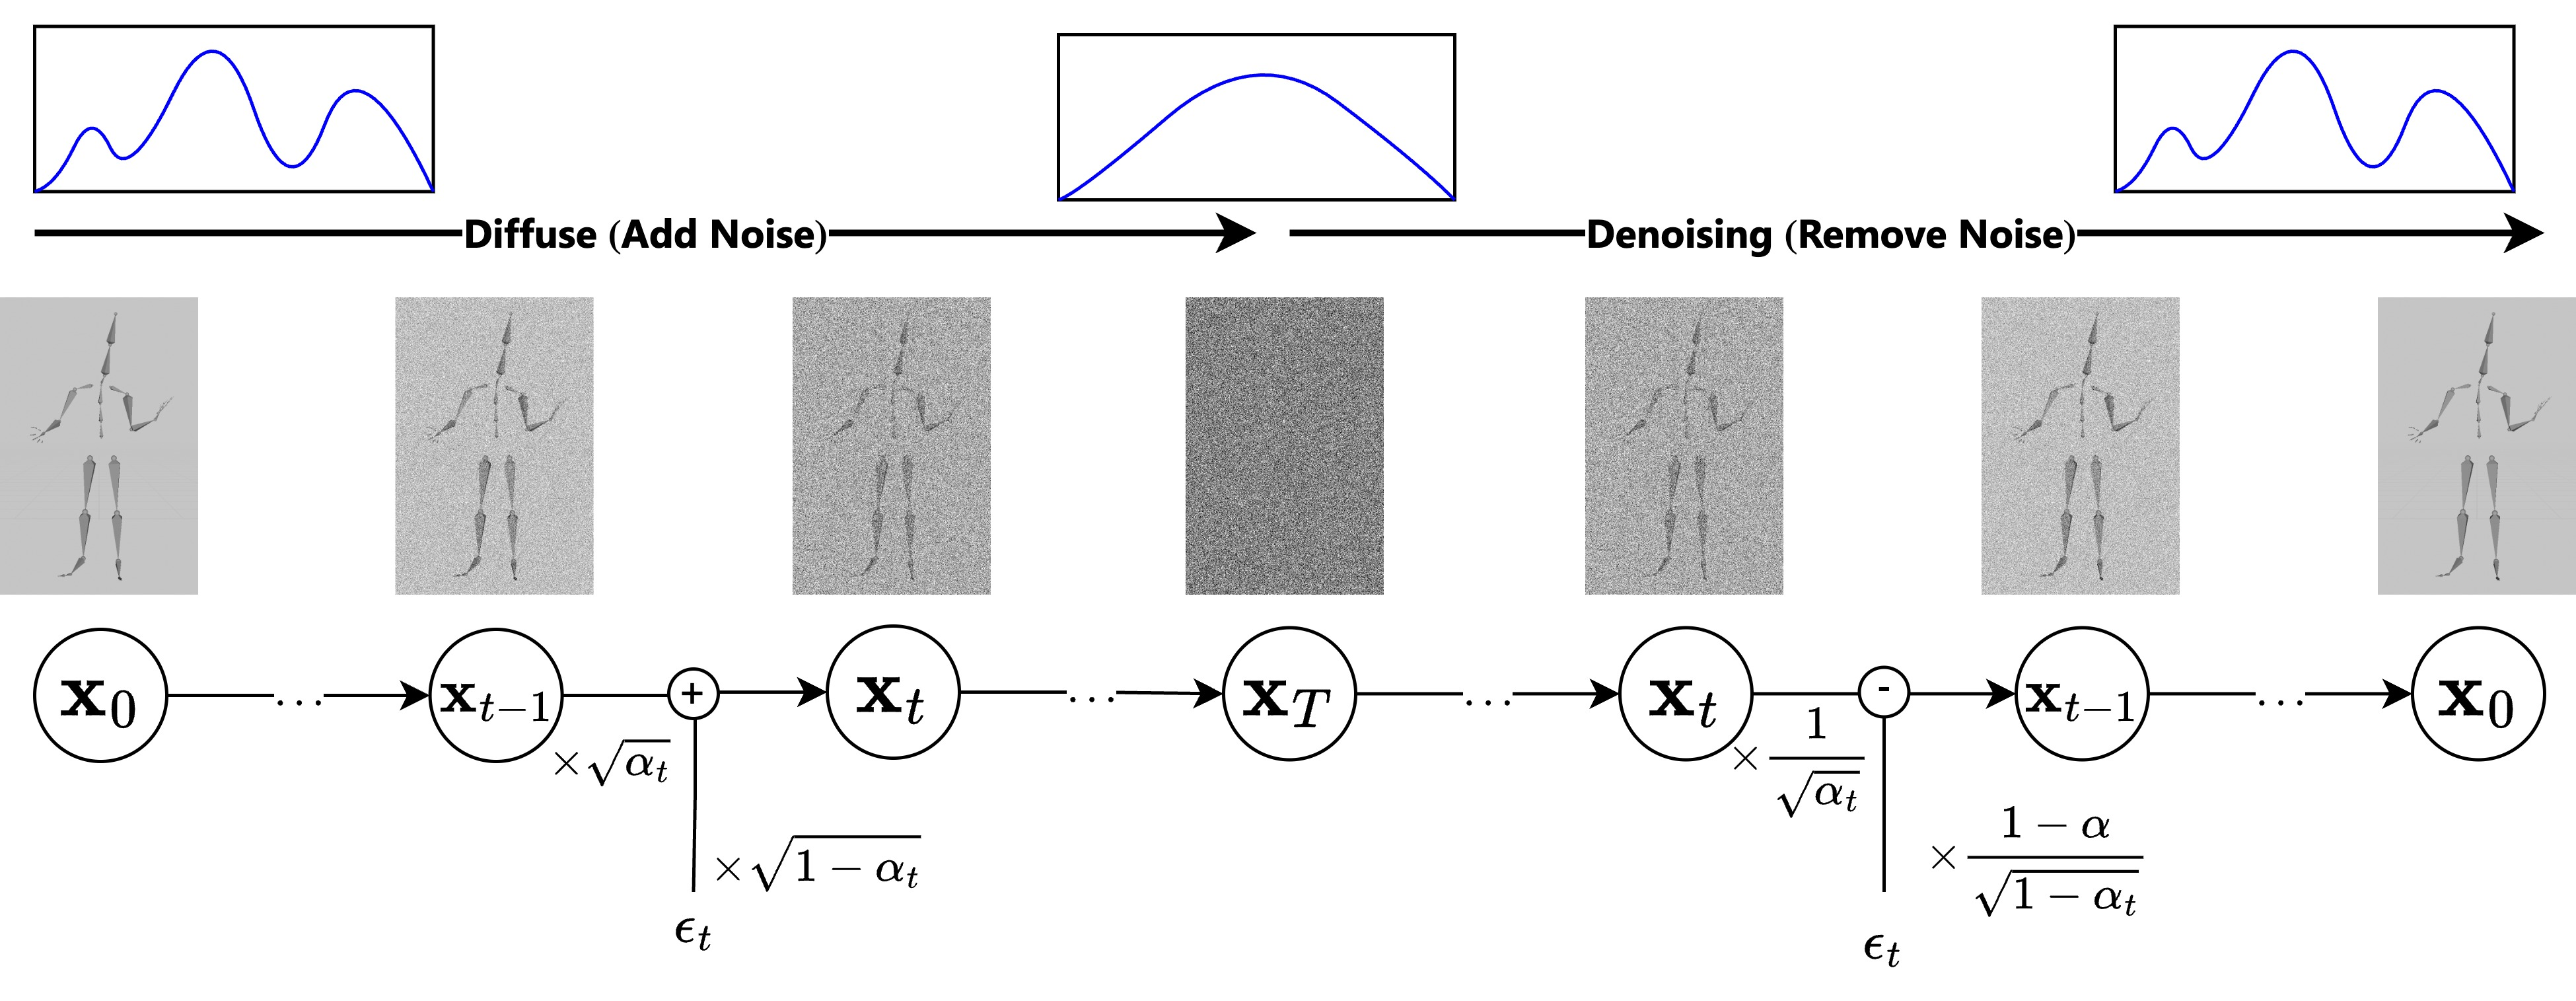
\includegraphics[width=\textwidth]{DiffuseAndDenoise.jpg}
    \end{figure}
    %\begin{equation}
    %	\mathbf{x}_{t-1}=\frac{1}{\sqrt{\alpha_t}}\left(\bx_t-\sqrt{1 - \alpha_t} \cdot \epsilon (\mathbf{x}_t, t )\right)
    %\end{equation}
    
    \begin{columns}
        \begin{column}{0.5\textwidth}
            \textbf{Denoise}
            \begin{equation}
                \mathbf{x}_{t-1} = \frac{1}{\sqrt{\alpha_{t}}} (\mathbf{x}_t - \sqrt{1- \alpha_t} \cdot \epsilon)
            \end{equation}
        \end{column}
        \begin{column}{0.5\textwidth}
        \begin{figure}
            \centering
            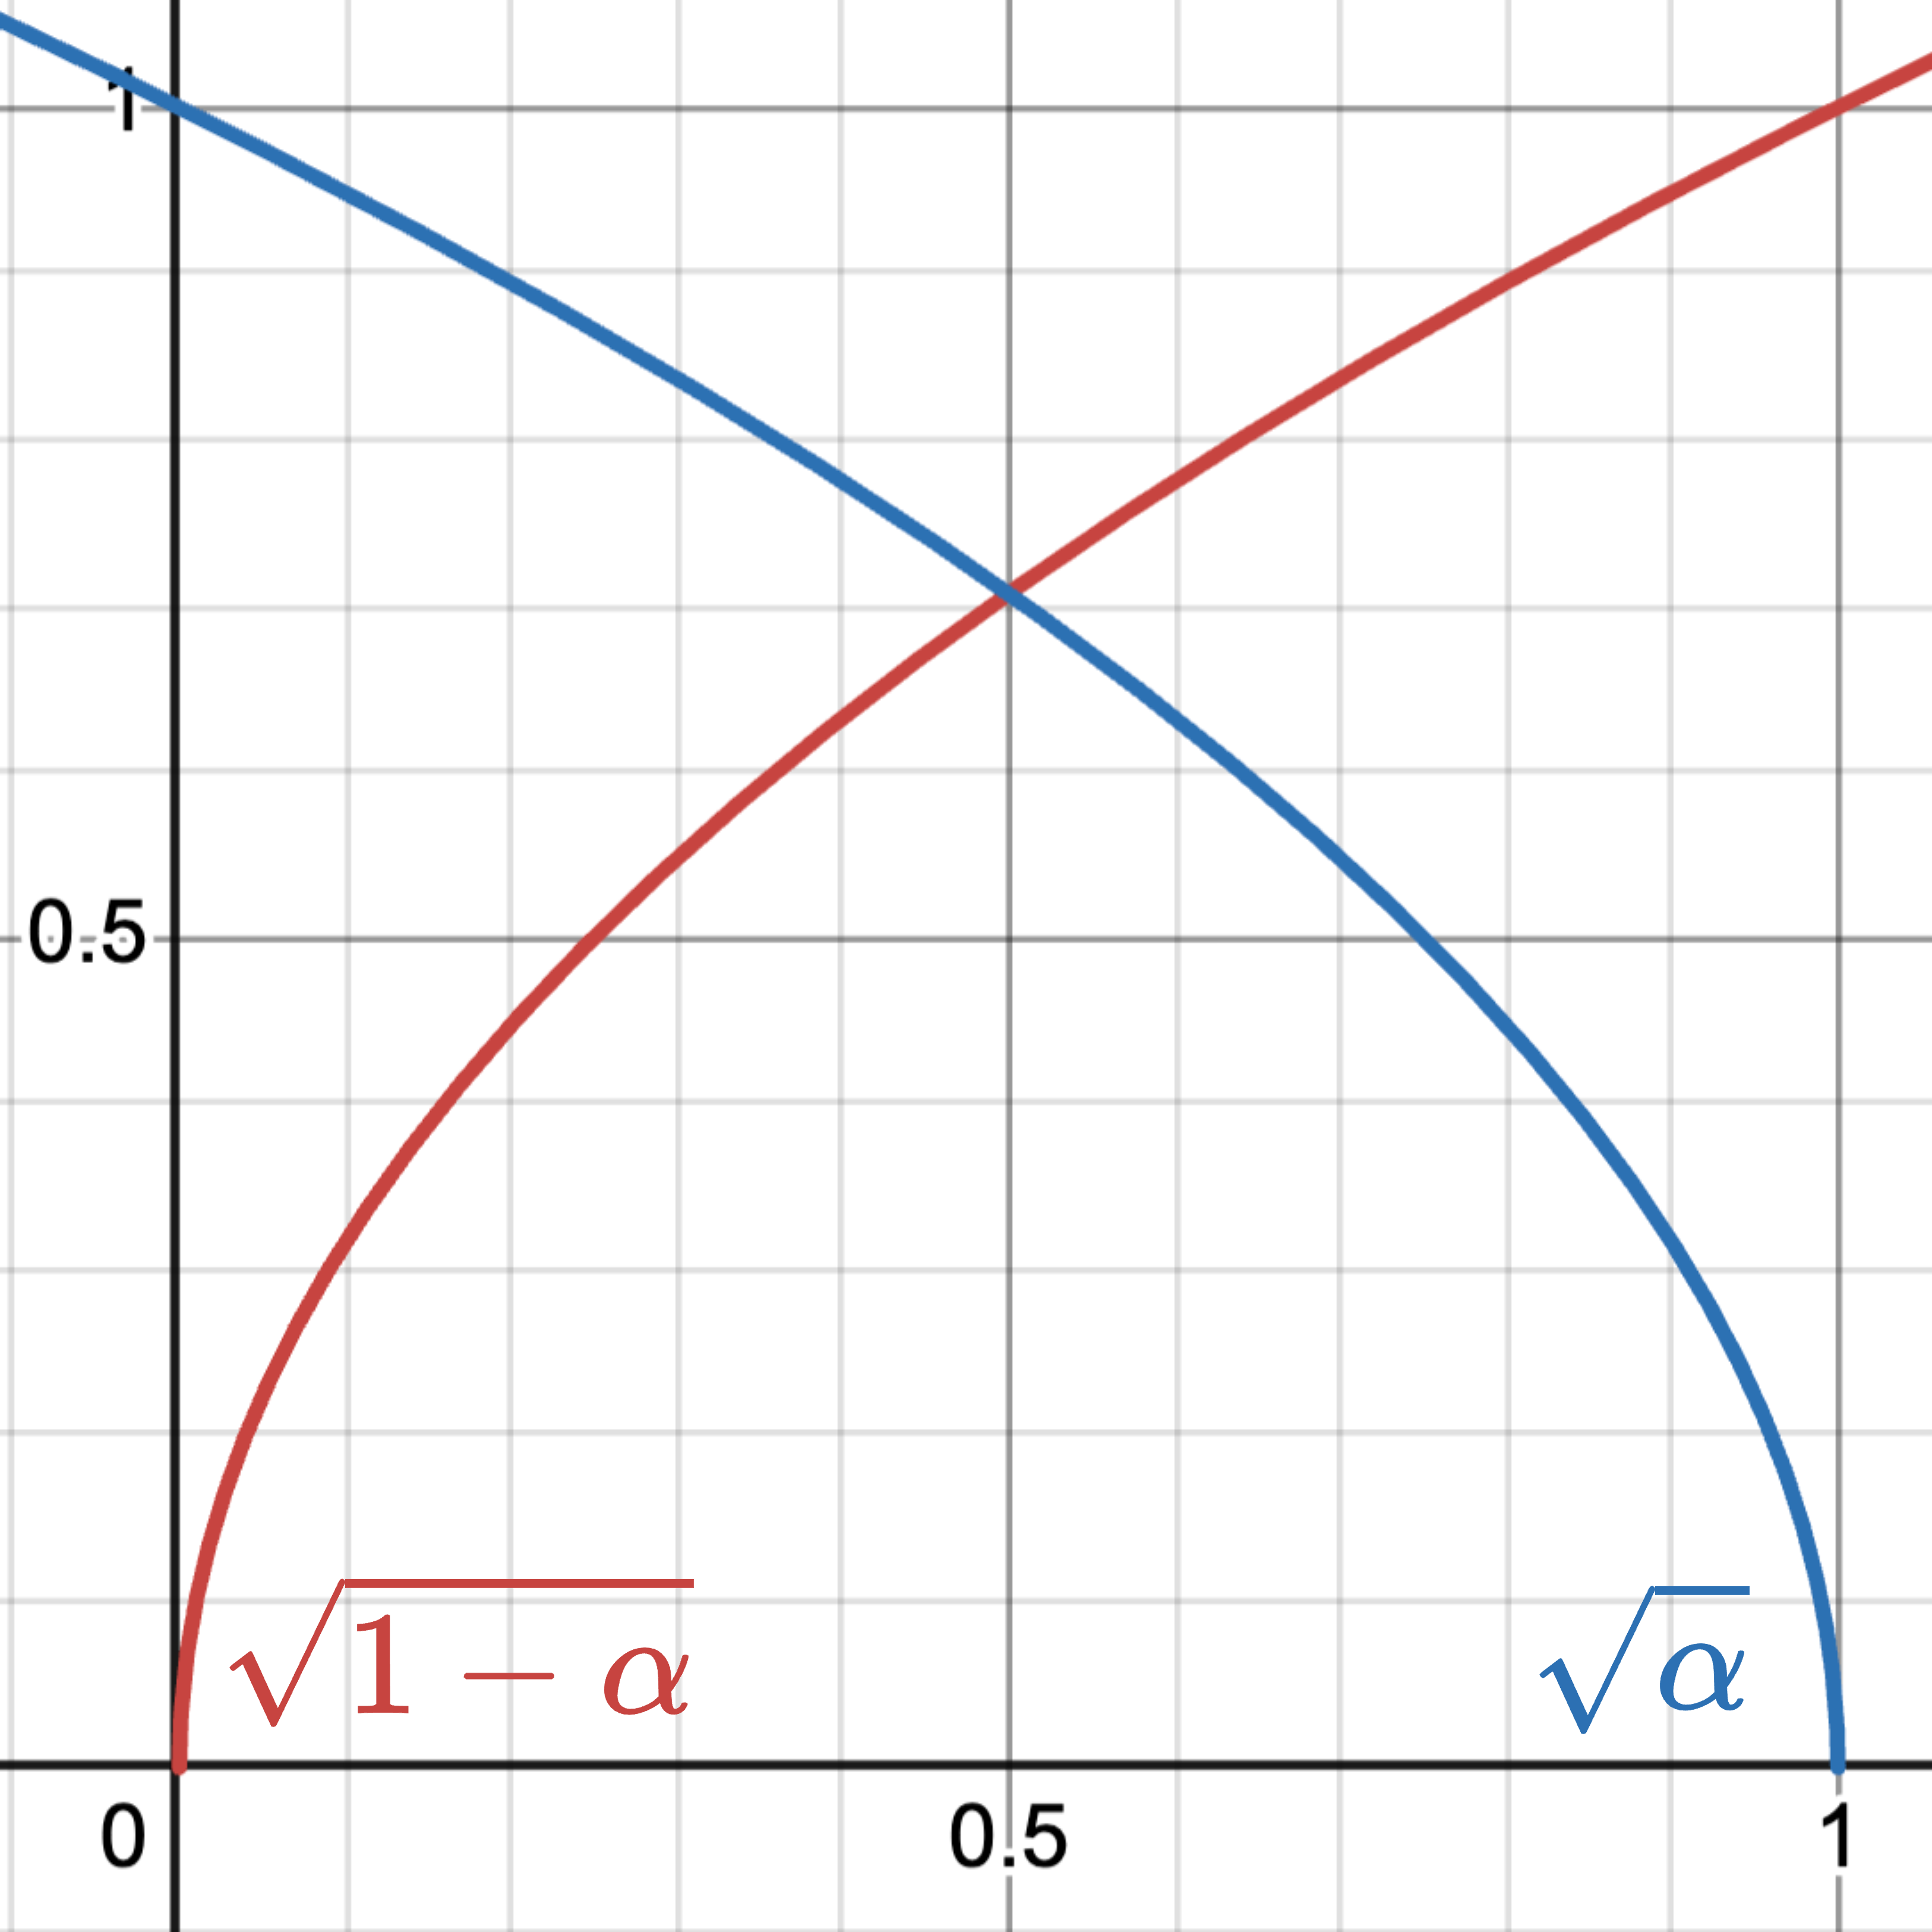
\includegraphics[width=0.4\textwidth]{SquareAlpha.png}
        \end{figure}
        \end{column}
    \end{columns}
    
    \end{frame}


\begin{frame}{Quan hệ $\bx_{0}$, $\bx_t$ và $\bx_{t - 1}$}
	
	Ta có thể suy ra $\bx_t$ từ $\bx_0$ và ngược lại. Với $ \boldsymbol{\epsilon}_{t-1}, \boldsymbol{\epsilon}_{t-2}, \dots \sim \mathcal{N}(\mathbf{0}, \mathbf{I})$
	%\begin{align*}
	%	\mathbf{x}_t & = \sqrt{\alpha_t}\mathbf{x}_{t-1} + \sqrt{1 - \alpha_t} \boldsymbol{\epsilon}_{t-1} \\
	%	& = \sqrt{\alpha_t \alpha_{t-1}} \mathbf{x}_{t-2} + \sqrt{1 - \alpha_t \alpha_{t-1}} \bar{\boldsymbol{\epsilon}}_{t-2} \\
	%	& = \dots \\
	%	& = \sqrt{\bar{\alpha}_t}\mathbf{x}_0 + \sqrt{1 - \bar{\alpha}_t}\boldsymbol{\epsilon}
	%\end{align*}
	\vspace{-10pt}
	
	\begin{figure}
		\centering
		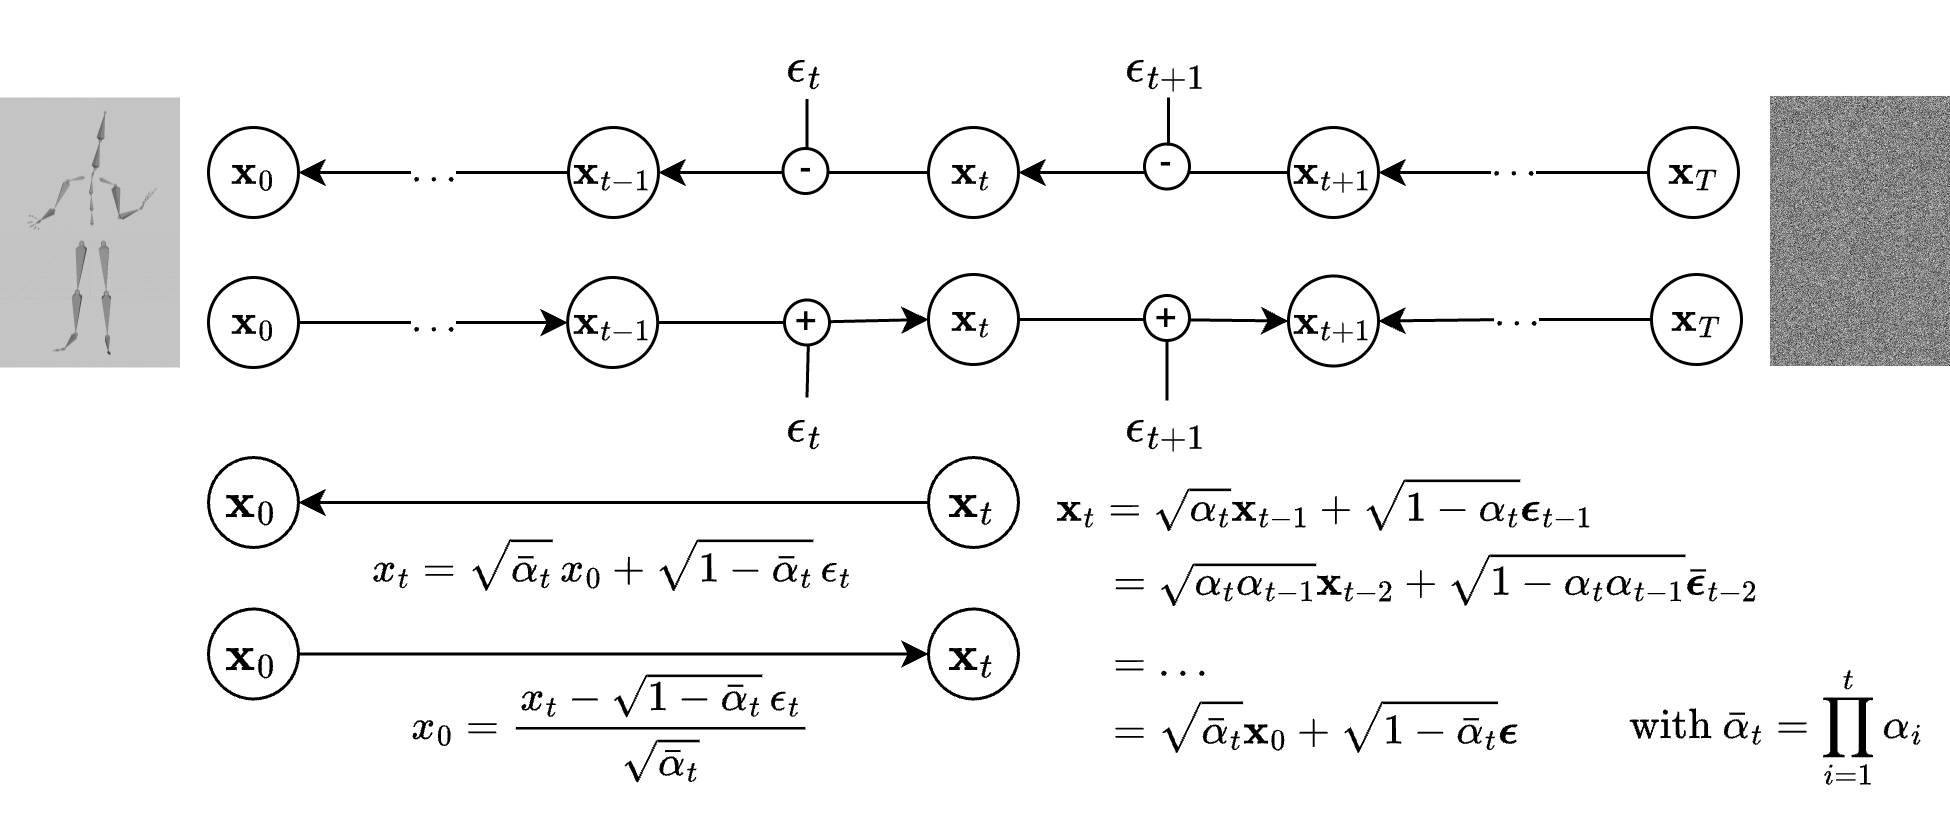
\includegraphics[width=\textwidth]{XRelation.png}
	\end{figure}
	%\vspace{-10pt}
	%	\mathbf{x}_t = \sqrt{\bar{\alpha}_t}\mathbf{x}_0 + \sqrt{1 - \bar{\alpha}_t}\boldsymbol{\epsilon}
	\begin{columns}
		\begin{column}{0.5\textwidth}
			\begin{itemize}
				\item $\bar{\alpha}_1 > \dots > \bar{\alpha}_T$
				\item Tổng hai nhiễu cũng là nhiễu:
				\footnotesize
				$$
				\mathcal{N}(\mathbf{0}, \sigma_1^2\mathbf{I}) + 
				\mathcal{N}(\mathbf{0}, \sigma_2^2\mathbf{I})
				=\mathcal{N}(\mathbf{0}, (\sigma_1^2 + \sigma_2^2)\mathbf{I})
				$$
			\end{itemize}
		\end{column}
		\begin{column}{0.5\textwidth}
			
			\begin{figure}
				\centering
				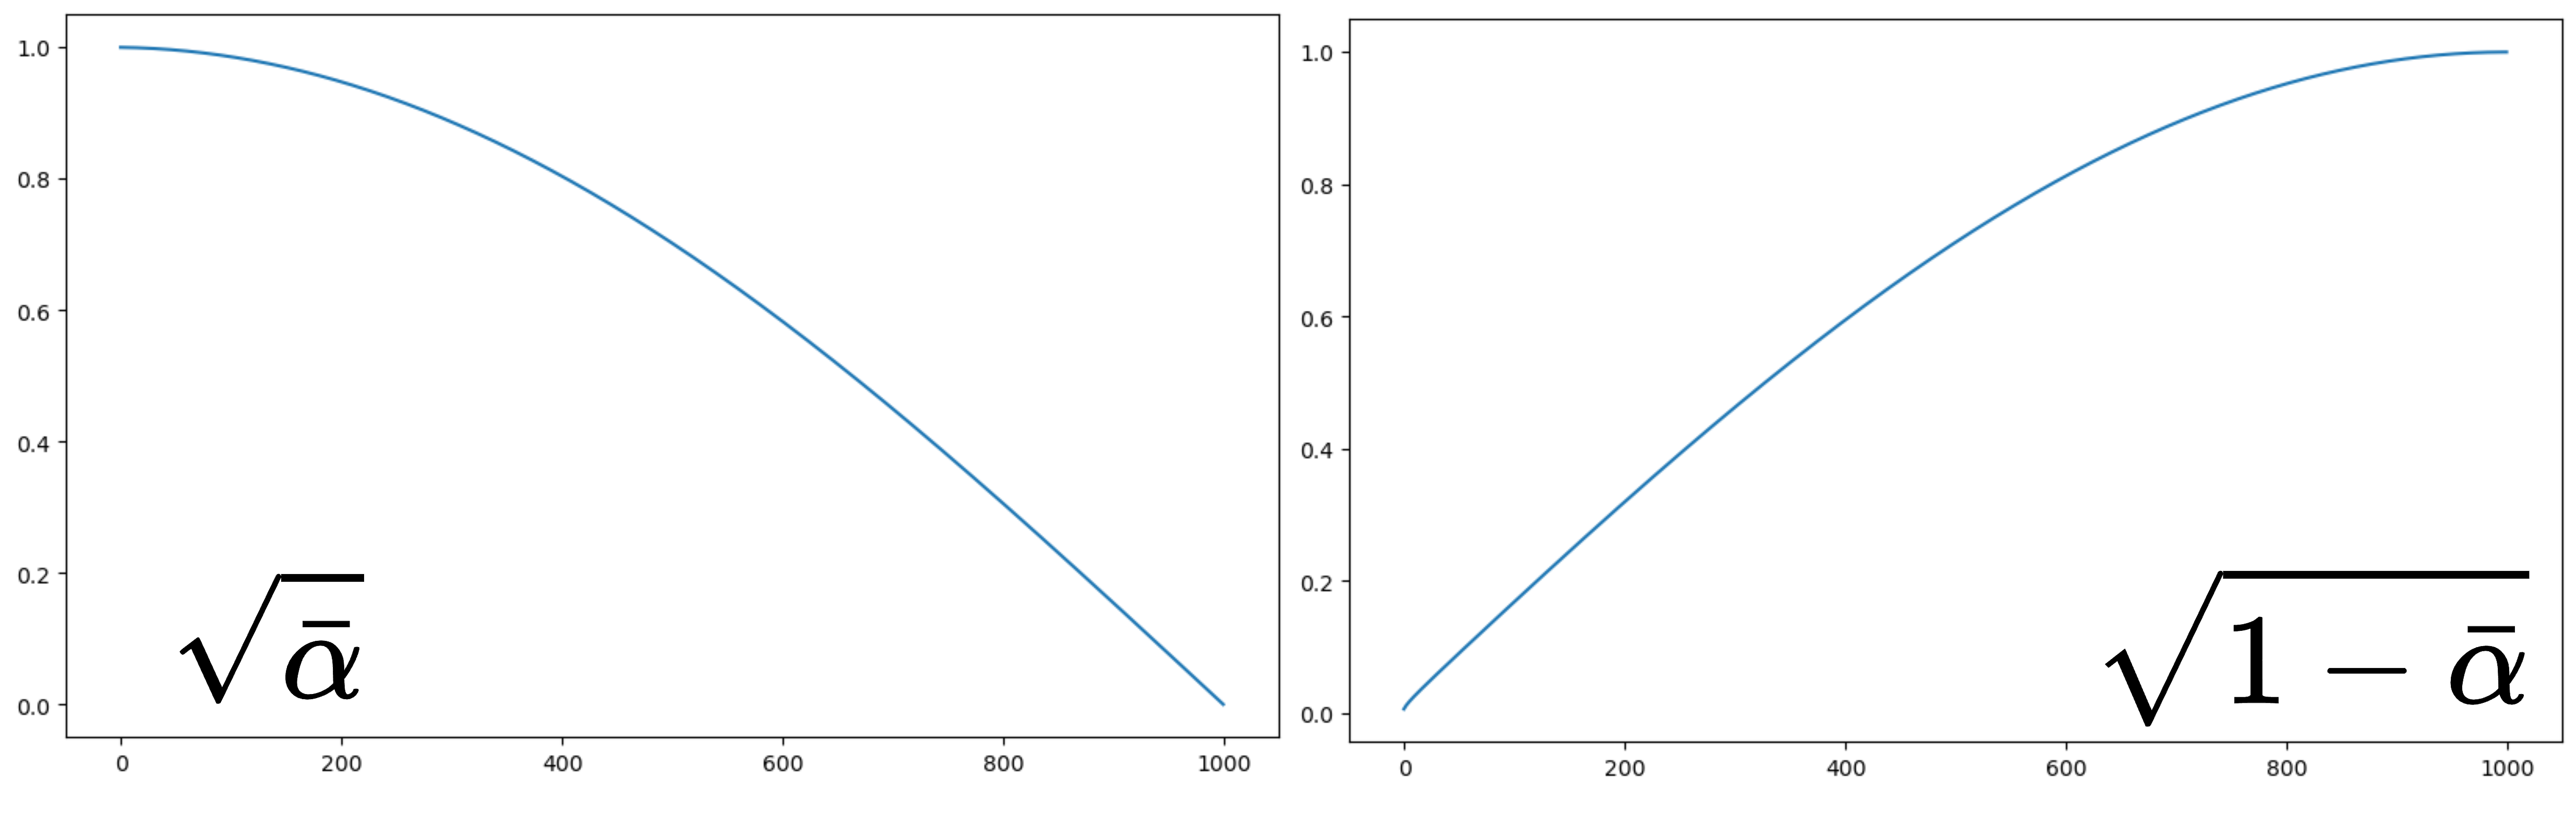
\includegraphics[width=\textwidth]{AlphaCumprod}
			\end{figure}
			
			
		\end{column}
	\end{columns}
	
\end{frame}


\begin{frame}{$q(\bx_t | \bx_{t-1})$ và $p_{\theta}(\bx_{t-1} | \bx_t ) $  trong DDPM }
	\textbf{DDPM} (Denoising Diffusion Probabilistic Model \cite{ho2020denoisingdiffusionprobabilisticmodels})
\begin{figure}
	\centering
	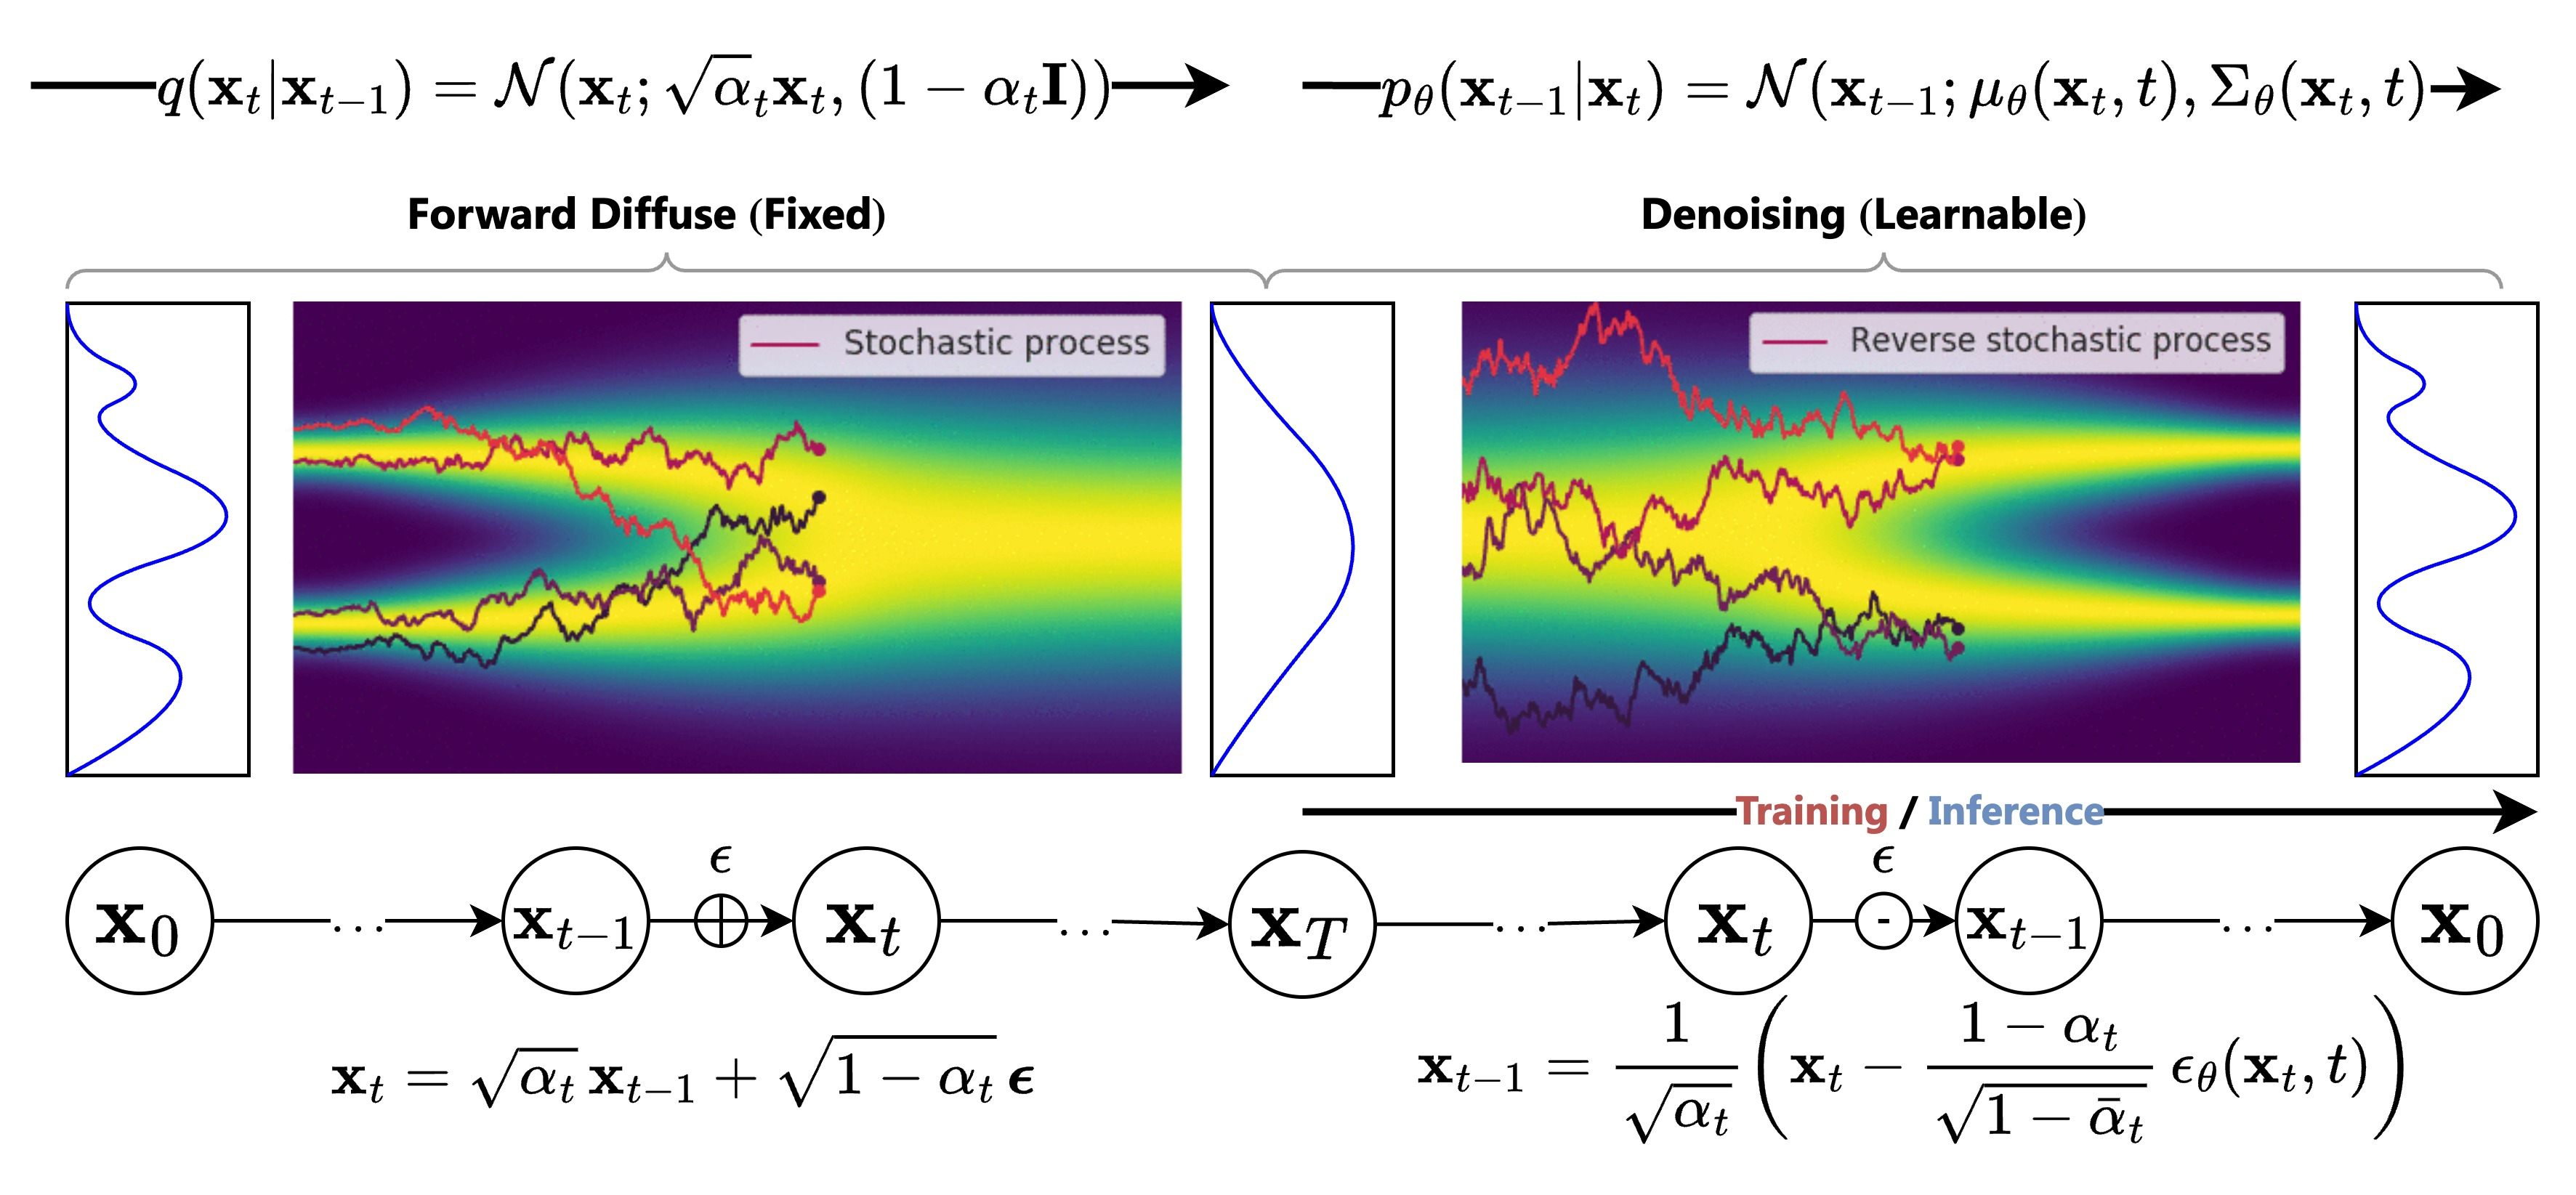
\includegraphics[width=\textwidth]{PQ}
\end{figure}
	
\begin{itemize}
	\item $q (\mathbf{x}_{t} | \mathbf{x}_{t-1}) = \mathcal{N}(\mathbf{x}_t; \sqrt{\alpha}_t \mathbf{x}_t, (1 - \alpha_t \mathbf{I}))$
	\item $p_\theta (\mathbf{x}_{t-1} | \mathbf{x}_{t}) = \mathcal{N}(\mathbf{x}_{t-1}; \mu_\theta{(\mathbf{x}_t, t)}, {\Sigma}_{\theta} {  (\mathbf{x}_t, t ) }$
\end{itemize}
%	$q(\mathbf{x}_t \vert \mathbf{x}_0) = \mathcal{N}(\mathbf{x}_t; \sqrt{\bar{\alpha}_t} \mathbf{x}_0, (1 - \bar{\alpha}_t)\mathbf{I})$
%
%
%
%\begin{equation}
%	\mathbf{x}_{t-1}=\frac{1}{\sqrt{1- \beta_t}}\left(\bx_t-\sqrt{\beta_t} \cdot \epsilon_{\color{red}{\theta}}\left(\mathbf{x}_t, t\right)\right)+\color{red}{\beta_t \cdot \sigma_t \mathbf{z}} \color{black}{}
%\end{equation}

\end{frame}

\begin{frame}{Vanilla Diffusion với $\epsilon$ Objective}
	\begin{figure}
		\centering
		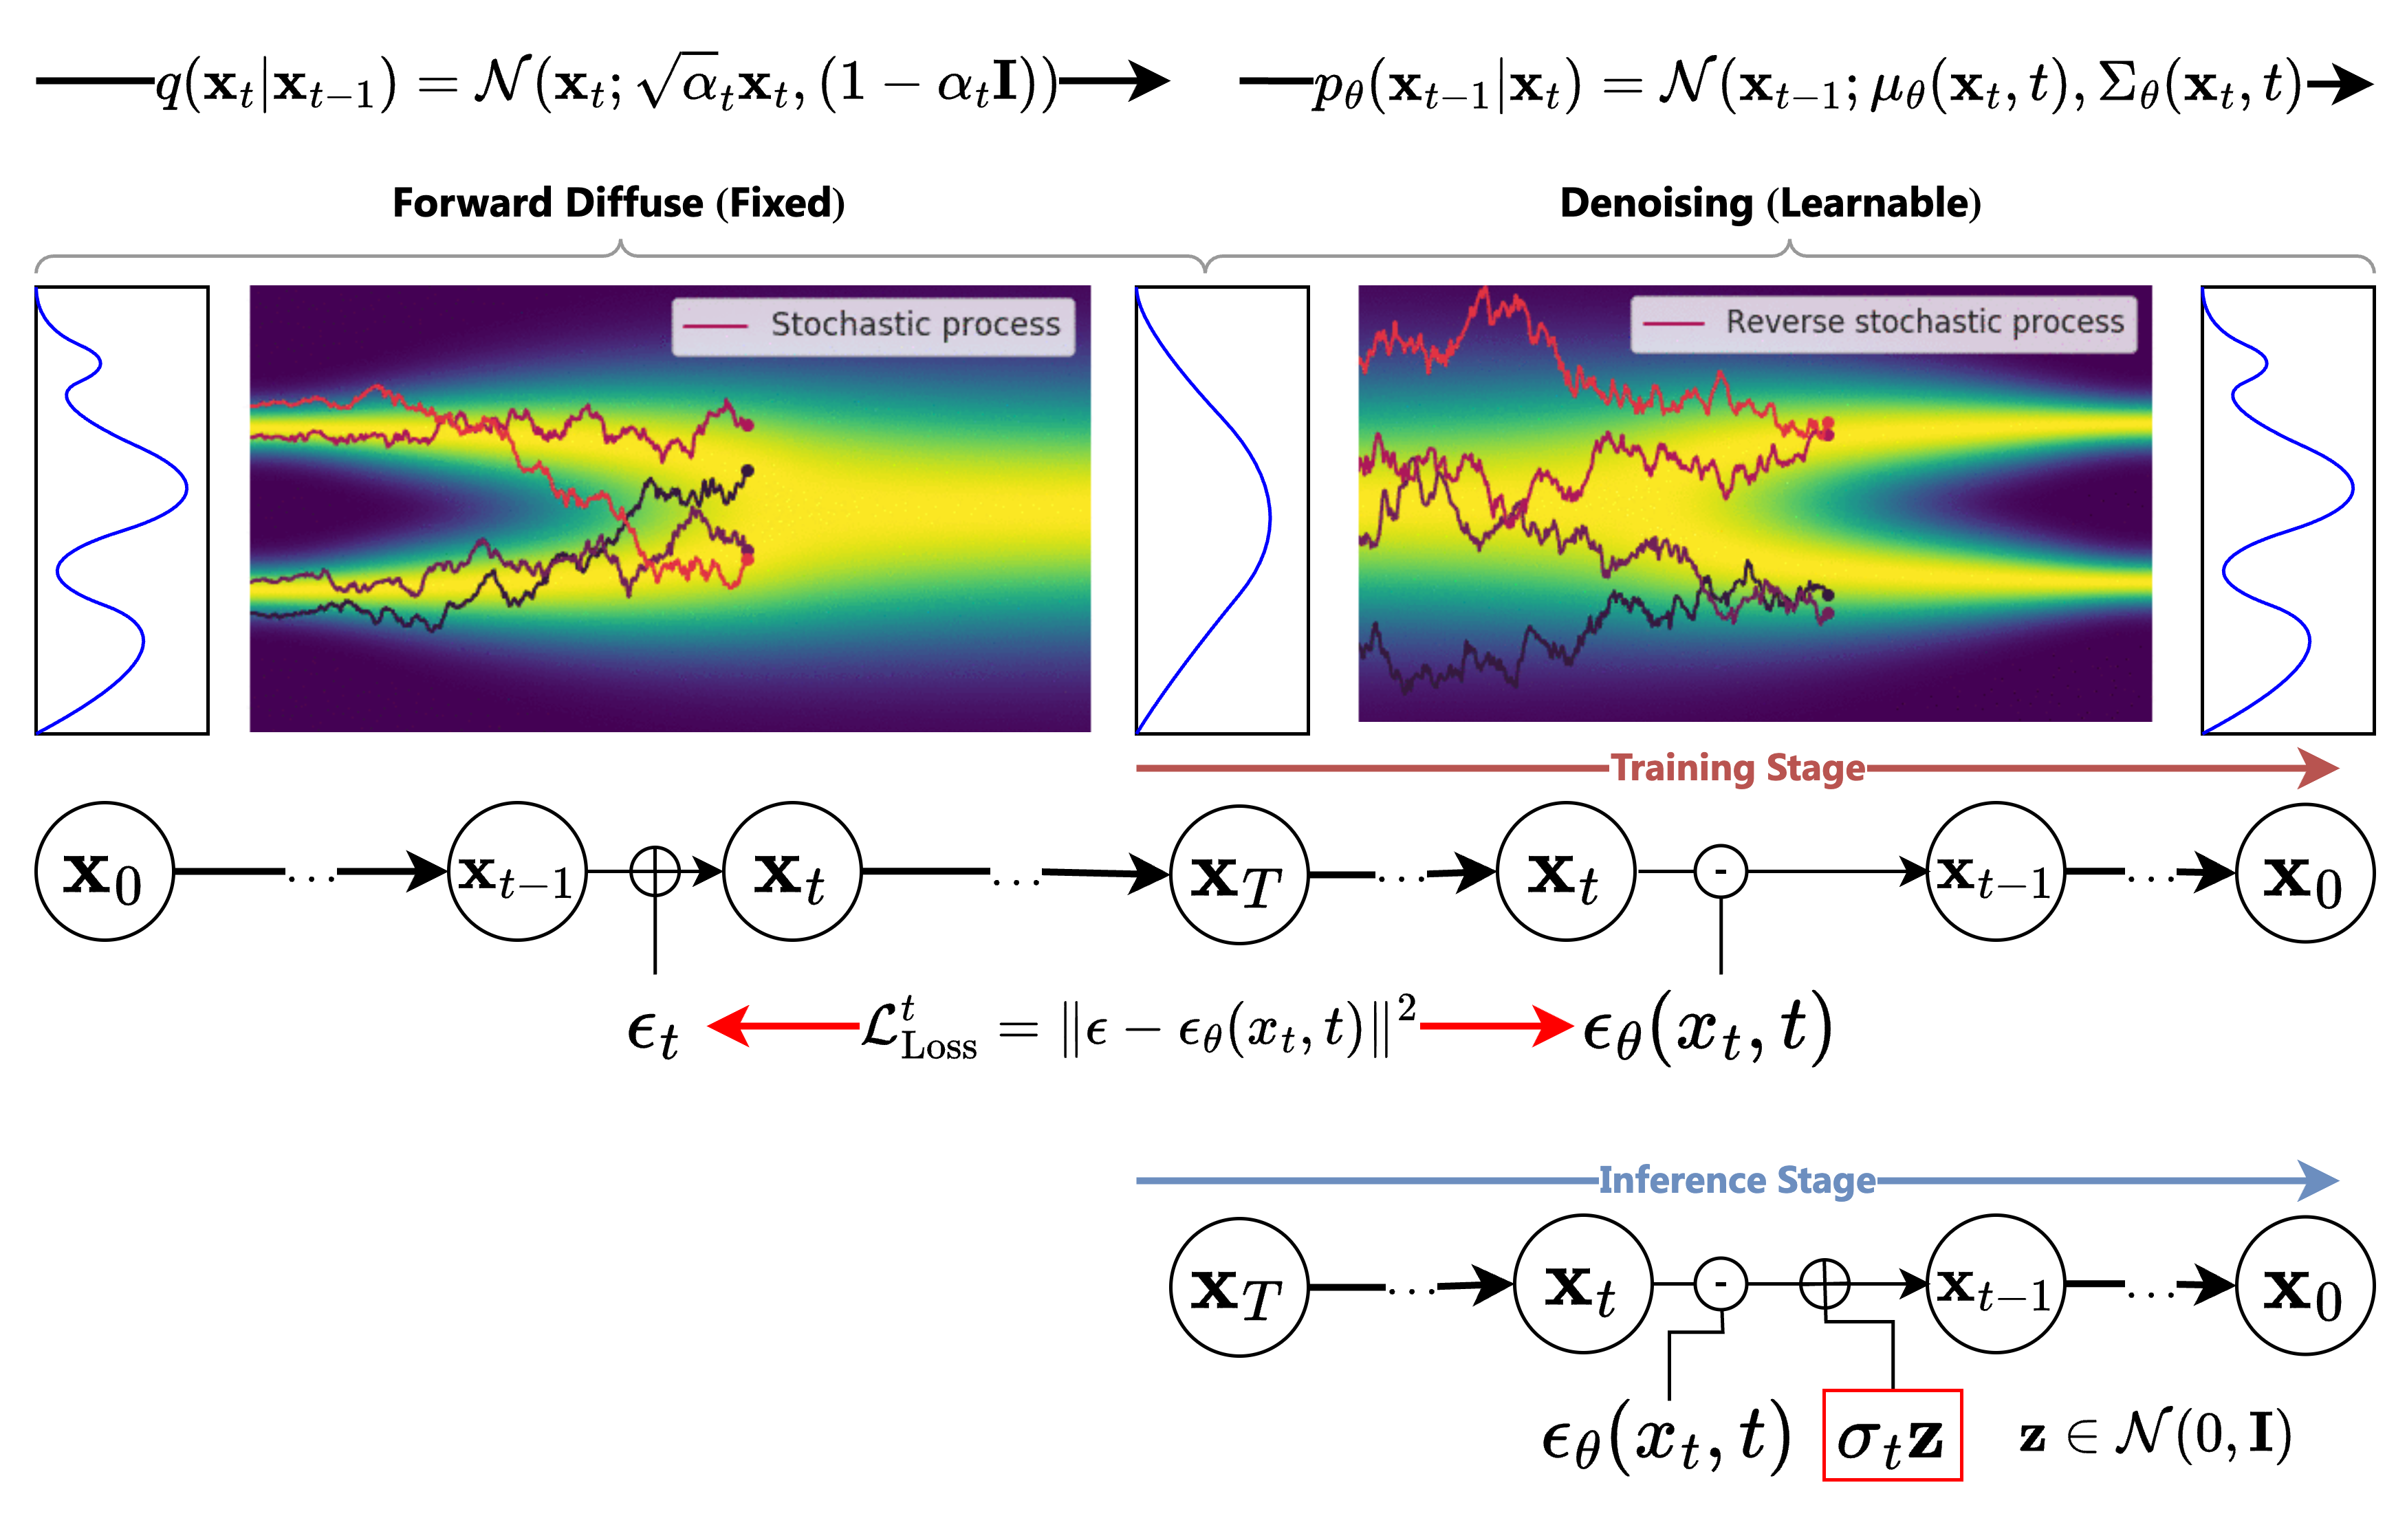
\includegraphics[width=0.95\textwidth]{TrainingAndSamplingStandard}
	\end{figure}
\end{frame}

\begin{frame}{Điều khiển $\sigma_t$ bằng với Langevin dynamics}
%	Cho $L$ là biến điều chỉnh độ lệch chuẩn
	%	 $\mathcal{N}(0, \sigma_i^2 I), i=1,2,\cdots,L$. $\mathbf{s}_\theta(\mathbf{x}, i) \approx \nabla_\mathbf{x} \log p_{\sigma_i}(\mathbf{x})$ $i= 1, 2, \cdots, L$.
	
%	Ta dễ dàng sinh mẫu (sampling) từ ${\sigma_i}(\mathbf{x})$ bằng cách lấy mẫu $\mathbf{x} \sim p(\mathbf{x})$  và tính $\mathbf{x} + \sigma_i \mathbf{z}$ với $\mathbf{z} \sim \mathcal{N}(0, I)$
Trong quá trình Denoise ($T \rightarrow 0$)  $\sigma_T > \cdots  >  \sigma_2 > \sigma_1$, ta sẽ giảm $\sigma_t$ để giảm dần nhiễu, để mô hình có thể hội tụ ở những vùng có mật độ xác xuất cao.
	\begin{figure}
		\centering
		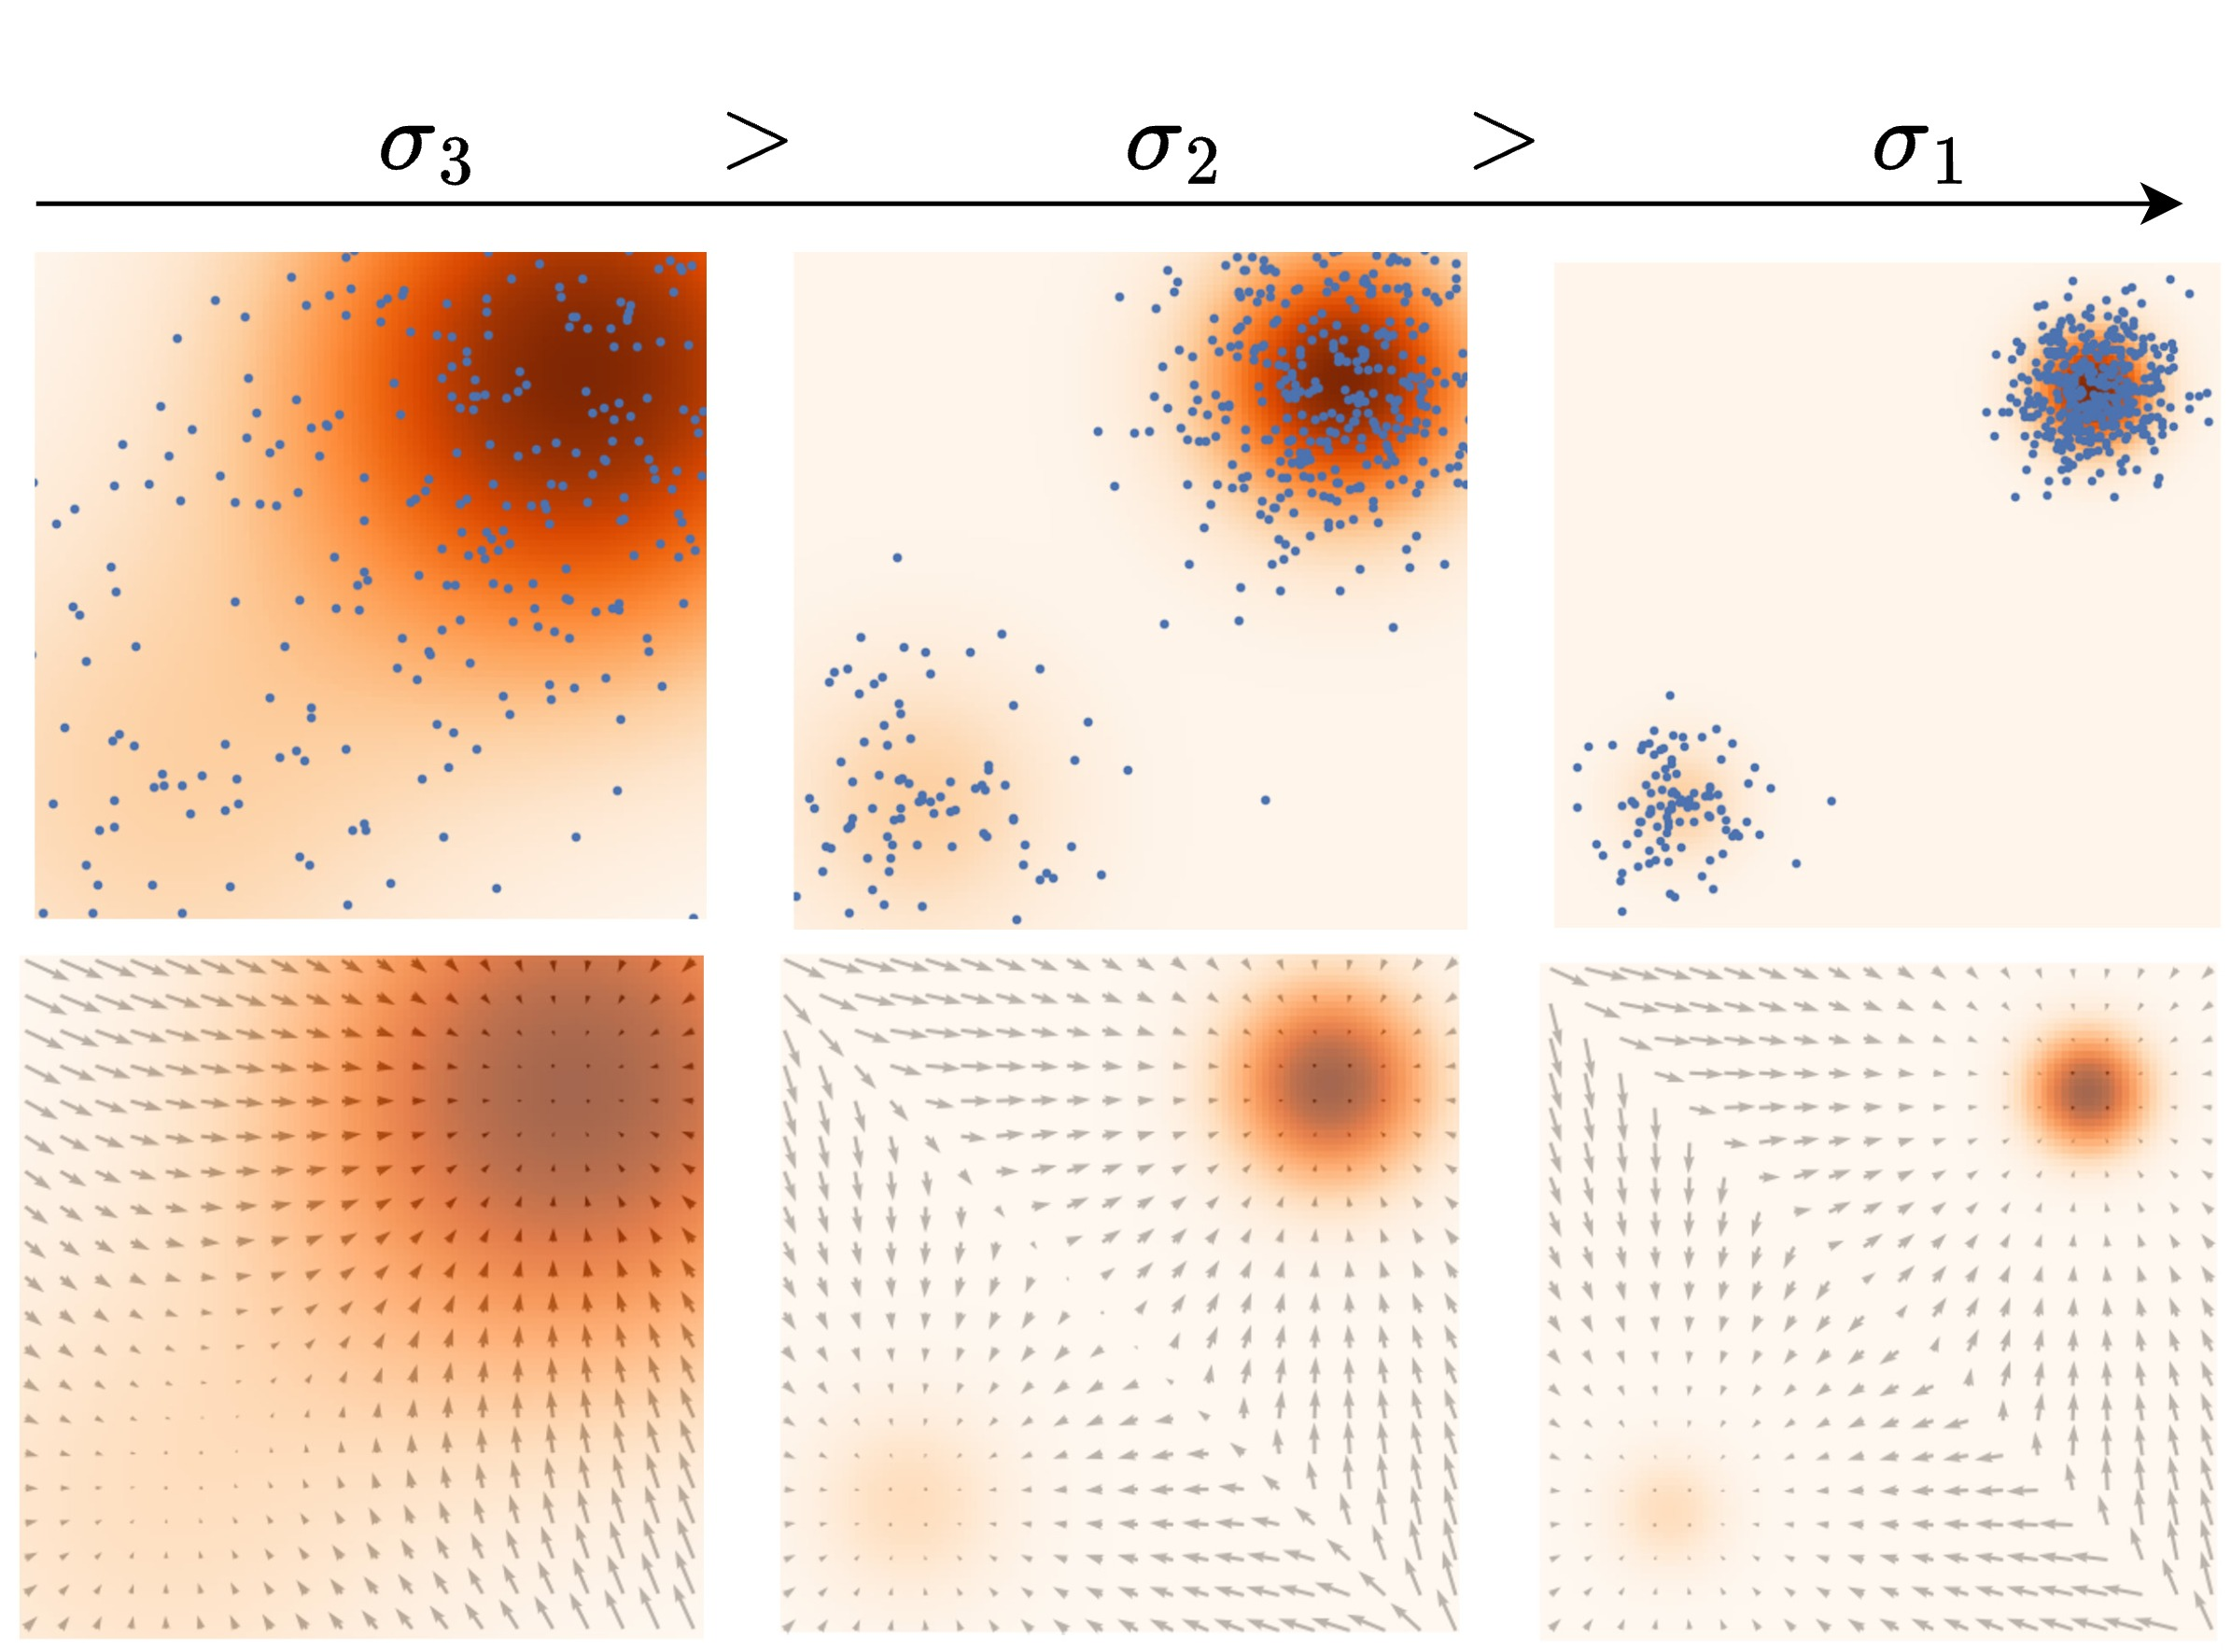
\includegraphics[width=0.8\linewidth]{NoiseScale.jpg}
	\end{figure}
\end{frame}

\begin{frame}{Training DDPM}
	\textbf{Hàm loss}: $\mathcal{L} = \sum_{t=1}^{T} \mathcal{L}_t$. $\mathcal{L}_{t}= \mathbb{E}_{\mathbf{x}_{0}, \epsilon_t \sim \mathcal{N}(0, I), t} \left[ \| \epsilon_t - \epsilon_\theta(\mathbf{x}_t, t) \|^2 \right]$
	
	\begin{figure}
		\centering
		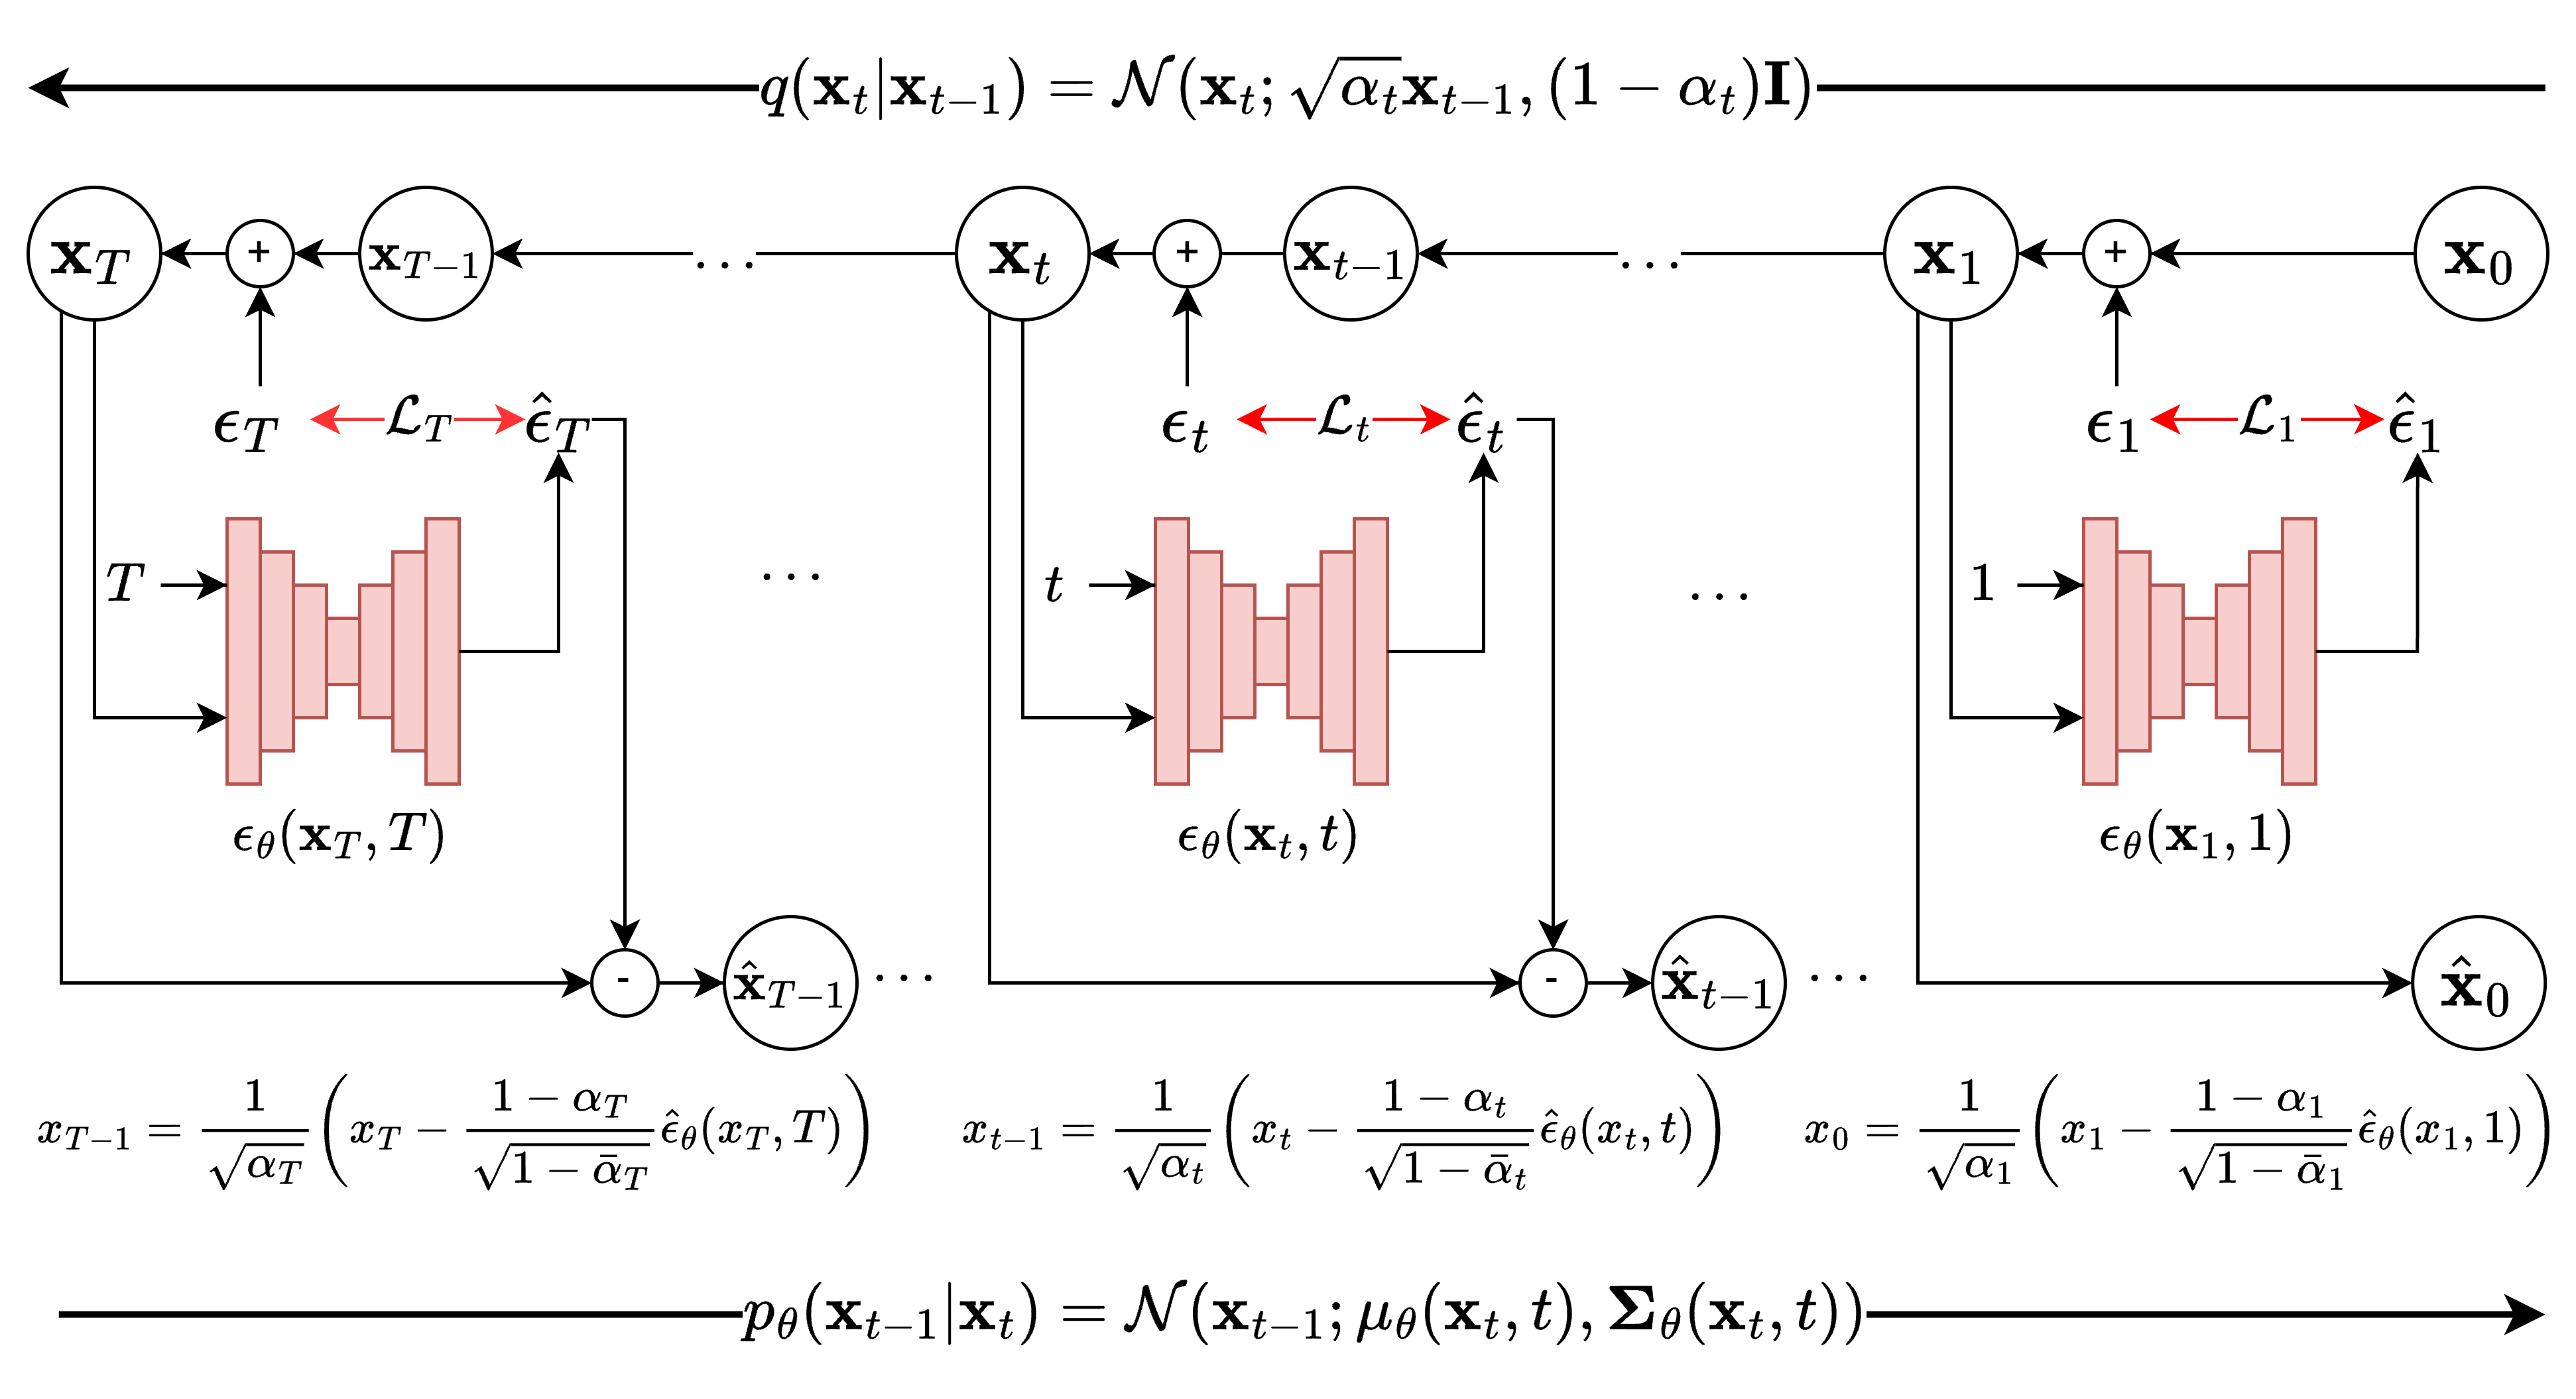
\includegraphics[width=\linewidth]{DDPMTraining}
	\end{figure}
\end{frame}

\begin{frame}{Các bước huấn luyện với DDPM}
	
	\begin{enumerate}
		\item Tính sẵn các giá trị $\sqrt{\alpha_t}$ $\sqrt{1 - \alpha_t}$ và $\sqrt{\bar{\alpha}_t}$ ở mọi bước $t: 1 \rightarrow T$.
		$\{\alpha_t \in (0, 1)\}_{t=1}^T$, $\alpha_1 < \alpha_2 < \dots < \alpha_T$
		\item Lấy nhãn $\bx_0$ từ phân bố của dữ liệu đã chuẩn hoá
		\item Random nhiễu $\bepsilon_t$ ở mọi bước $t: 1 \rightarrow T$, với  $\forall t:  \bepsilon_t \sim\mathcal{N}(\bzero,\bI)$
		\item Gây nhiễu (forward) $\bx_0$ để thu được $\bx_t$ ở mọi bước $t: 1 \rightarrow T$
		$$
		\mathbf{x}_t = \sqrt{\bar{\alpha}_t}\mathbf{x}_0 + \sqrt{1 - \bar{\alpha}_t}\boldsymbol{\epsilon}_t
		$$
		\item $\text{for all}$ $t$, lẫy $t$ \textbf{ngẫu nhiên} $t \sim [1, T]$
		\item Cho $\bx_t$ và $t$ vào mô hình để dự đoán nhiễu $\hat{\bepsilon} = \bepsilon_\theta(\mathbf{x}_t, t)$
		\item Đạo hàm để cập nhật trọng số $\qquad \grad_{\theta_t} \left\| \bepsilon_t - \bepsilon_\theta(\mathbf{x}_t, t) \right\|^2$
		$$
			\mathcal{L}_t = \mathbb{E}_{t \sim [1, T], \mathbf{x}_0, \boldsymbol{\epsilon}_t} \Big[\|\boldsymbol{\epsilon}_t - \boldsymbol{\epsilon}_\theta(\sqrt{\bar{\alpha}_t}\mathbf{x}_0 + \sqrt{1 - \bar{\alpha}_t}\boldsymbol{\epsilon}_t, t)\|^2 \Big]
		$$
		\item Quay lại bước 6 cho đến khi hội tụ để thu được $\theta'$
	\end{enumerate}
\end{frame}

\begin{frame}{Sampling DDPM}
	\textbf{Hàm sampling}:
	\begin{itemize}
		\item $\bx_T \in \mathcal{N}(0, \mathbf{I})$
	\end{itemize}
	
	\begin{equation*}
		x_{t-1} = \frac{1}{\sqrt{\alpha_t}} \left( x_t - \frac{1 - \alpha_t}{\sqrt{1 - \bar{\alpha}_t}} \hat{\epsilon}_{\theta'}(x_t, t) \right) + \sigma_t \mathbf{z}
	\end{equation*}
	
	\begin{itemize}
		\item Diffusion: $\mathcal{L}_{\text{loss}}= \mathbb{E}_{\mathbf{x}_{0}, \epsilon_t \sim \mathcal{N}(0, I), t} \left[ \| \epsilon_t - \epsilon_\theta(\mathbf{x}_t, t) \|^2 \right]$
	\end{itemize}
	\begin{figure}
		\centering
		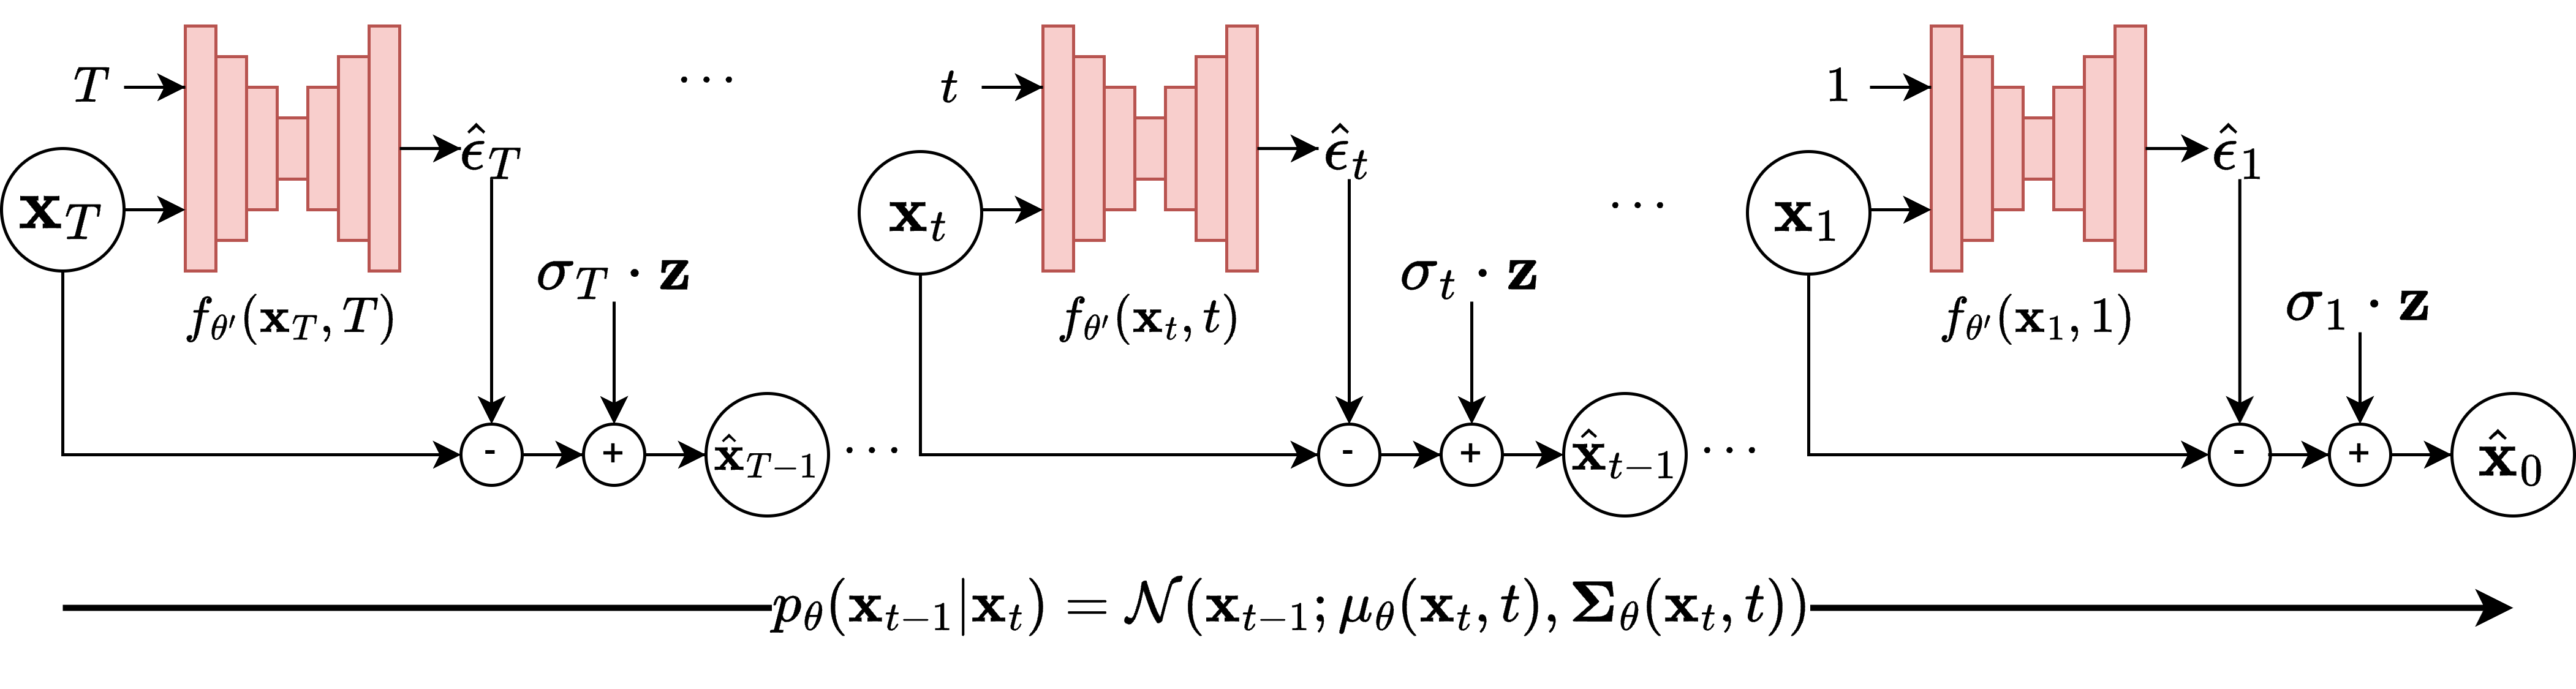
\includegraphics[width=\linewidth]{DDPMSampling}
	\end{figure}
\end{frame}

\begin{frame}{Các bước lấy mẫu với DDPM}
	
	\begin{enumerate}
		\item Bắt đầu với nhiễu: $\bx_T \sim \mathcal{N}(0, \mathbf{I})$
		\item Các giá trị $\sqrt{\alpha_t}$ $\sqrt{1 - \alpha_t}$ và $\sqrt{\bar{\alpha}_t}$ có được từ bước huấn luyện
		\item Tính hệ số điều chỉnh nhiễu $\sigma_t$ từ $\alpha_t$ ở mọi bước $t: 1 \rightarrow T$
		$\sigma_t = \sqrt{\frac{1 - \bar{\alpha}_{t-1}}{1 - \bar{\alpha}_t} (1 - \alpha_t)}$
		
		\item $\text{for all}$ $t$, lấy $t$ \textbf{tuần tự} $t \sim [T, \dots 1]$
		\item Random nhiễu $\bz \sim \mathcal{N}(0, \mathbf{I})$
		\item Đưa $\bx_t$ vào để suy luận nhiễu $\bepsilon_{\theta'} = \bepsilon_{\theta'}(\bx_t, t)$
		\item Dùng nhiễu dự đoán để trừ đi $\bx_t$ ở bước $t$
			$$\mu =  \frac{1}{\sqrt{\alpha_t}}\left( \bx_t - \frac{1-\alpha_t}{\sqrt{1-\bar\alpha_t}} \bepsilon_{\theta'}(\bx_t, t) \right)$$
%			\hat{\bx}_{t-1} =
		\item Cộng thêm một lượng nhiễu $\hat{\bx}_{t-1} = \mu + \sigma_t \bz$
		\item Khi $t=1$ ta thu được $\hat{\bx}_0$ từ quá trình khử nhiễu
	\end{enumerate}
\end{frame}